\section{1174079 - Chandra Kirana Poetra}
\subsection{Teori}
\begin{enumerate}
	\item Jelaskan kenapa kata-kata harus di lakukan vektorisasi. Dilengkapi dengan ilustrasi atau gambar.
	\hfill\break
	Karena machine learning tidak akan mengerti tentang data yang akan diproses yaitu kata kata, oleh karena itu proses vektorisasi diperlukan sebelumnya untuk menerjemahkan kata kata tadi ke suatu value yang mesin bisa mengerti agar nantinya dapat diproses oleh mesin
	\hfill\break
	\begin{figure}[H]
		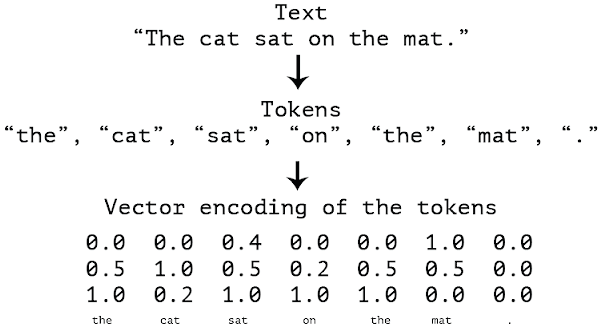
\includegraphics[width=7cm]{figures/1174079/5/1.png}
		\centering
		\caption{Teori 1}
	\end{figure}

	\item Jelaskan mengapa dimensi dari vektor dataset google bisa sampai 300. Dilengkapidengan ilustrasi atau gambar.
	\hfill\break
    Dataset yang didapatkan dari google bisa mencapai dimensi hingga 300 karena vektor yang ada digunakan sebagai perbandingan untuk memberi bobo daru suatu kata
    seperti misalkan yaitu kata dog dan juga cat yang ada pada dataset memiliki masing masing 300 dimensi vektor kemudian dibandingkan kesamaan katanya maka akan muncul
    hasil sekitar 70\% kesamaan bobot karena keduanya sama sama kata yang digunakan untuk hewan peliharaan.
	\hfill\break
	\begin{figure}[H]
		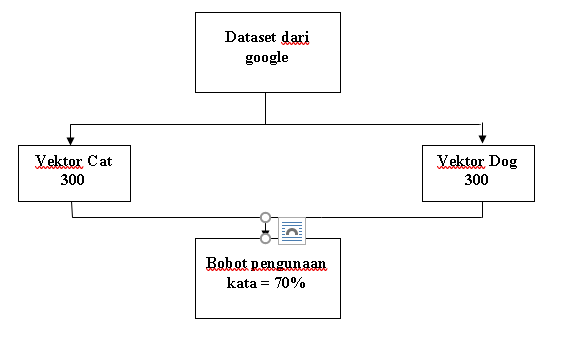
\includegraphics[width=7cm]{figures/1174079/5/2.png}
		\centering
		\caption{Teori 2}
	\end{figure}

	\item Jelaskan konsep vektorisasi untuk kata dilengkapi dengan ilustrasi atau gambar.
	\hfill\break
	Vektorisasi kata merupakan suatu metodologi dalam natural language processing untuk melakukan pemetaan 
    kata atau kalimat dari vocabulary menjadi suatu vektor dari angka yang digunakan untuk mencari prediksi kata atau sinonim
	\hfill\break
	\begin{figure}[H]
		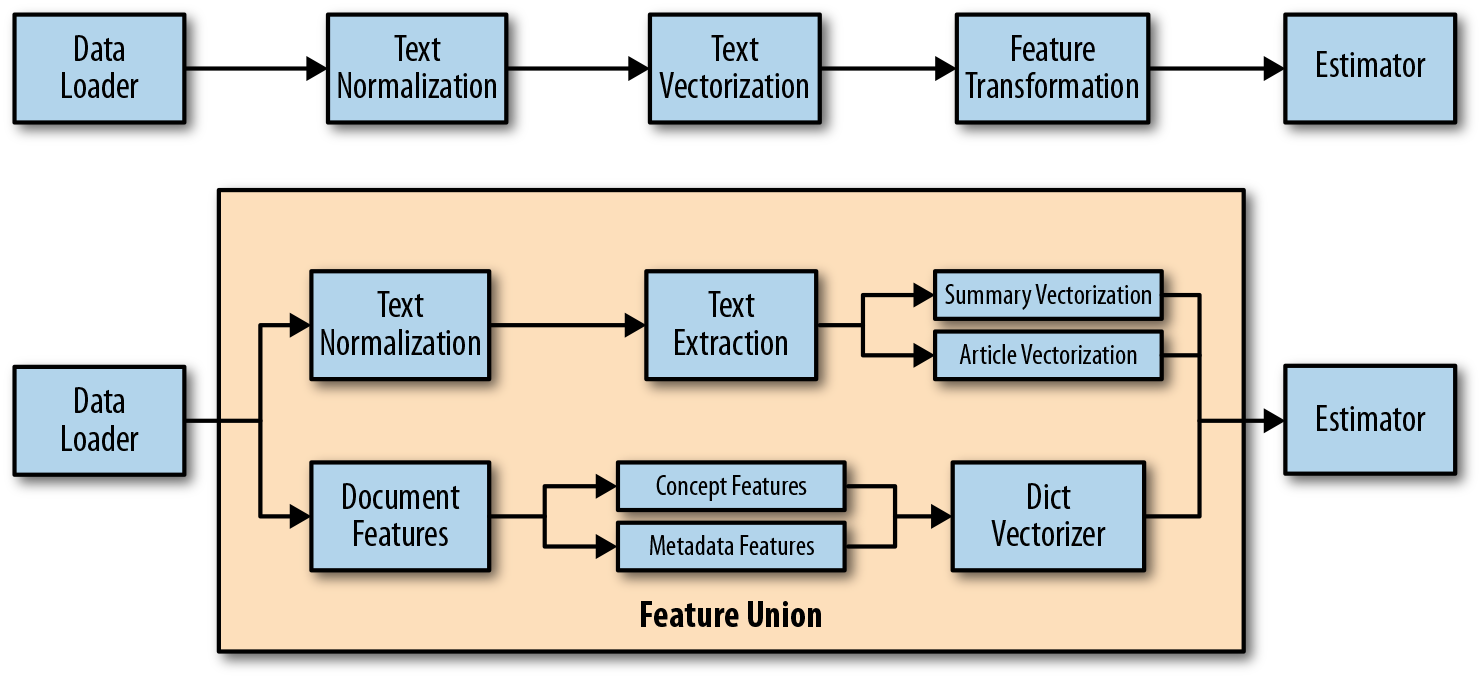
\includegraphics[width=7cm]{figures/1174079/5/3.png}
		\centering
		\caption{Teori 3}
	\end{figure}

	\item Jelaskan konsep vektorisasi untuk dokumen dilengkapi dengan ilustrasi atau gambar.
	\hfill\break
	Tujuan utama dari vektorisasi dokumen adalah sama seperti vektorisasi data yaitu untuk merepresentasikan karekter unik dari suatu dokumen secara numerical sehingga komputer bisa memproses suatu data teks yang tidak terstruktur
	\hfill\break
	\begin{figure}[H]
		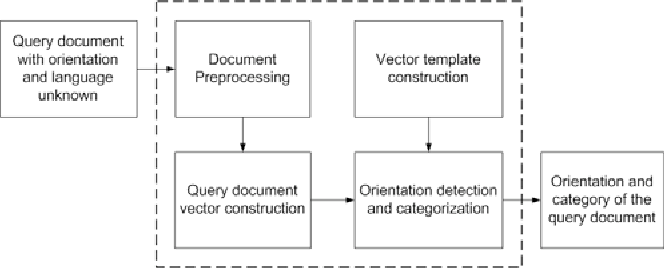
\includegraphics[width=7cm]{figures/1174079/5/4.png}
		\centering
		\caption{Teori 4}
	\end{figure}

	\item Jelaskan apa mean dan standar deviasi,dilengkapi dengan ilustrasi atau gambar.
	\hfill\break
    mean merupakan suatu hitungan yang menunjukkan seberapa sering suatu kata itu muncul . sedangkan standar deviasi merupakan suatu perhitungan pada statistik yang digunakan untuk menjelaskan homogenitas dari suatu data.
	\hfill\break
	\begin{figure}[H]
		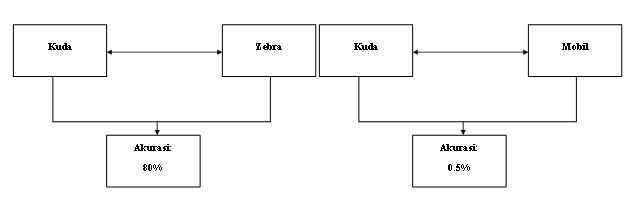
\includegraphics[width=7cm]{figures/1174079/5/5.png}
		\centering
		\caption{Teori 5}
	\end{figure}

	\item Jelaskan apa itu skip-gram,dilengkapi dengan ilustrasi atau gambar.
	\hfill\break
	Skip gram digunakan untuk memprediksi konteks kata untuk suata kata yang diberikan.
	\hfill\break
	\begin{figure}[H]
		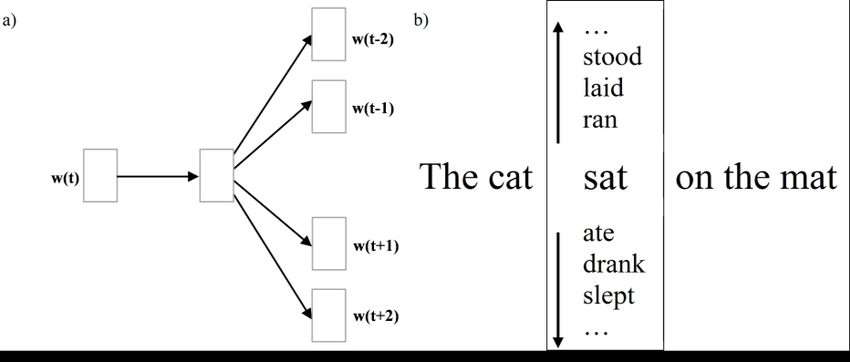
\includegraphics[width=7cm]{figures/1174079/5/6.png}
		\centering
		\caption{Teori 6}
	\end{figure}
\end{enumerate}
\subsection{Praktek}
\begin{enumerate}
	\item Cobalah dataset google, dan jelaskan vektor dari kata love, faith, fall, sick, clear,shine, bag, car, wash, motor, cycle dan cobalah untuk melakukan perbandingan similirati dari masing-masing kata tersebut.
	\begin{itemize}
		\item Import terlebih dahulu gensim serta logging, gensim untuk membuat data model sedangkan logging untuk melakukan logging kemudian load file bin google dengan memasukannya ke variable dengan limit 50000 dan juga binary true yang mengartikan bahwa file ini binary
		\hfill\break
	\lstinputlisting[firstline=10, lastline=12]{src/1174079/5/1174079.py}	
		\begin{figure}[H]
			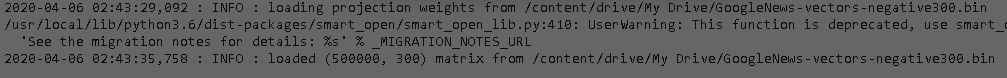
\includegraphics[width=7cm]{figures/1174079/5/7.png}
			\centering
			\caption{Praktek 1}
		\end{figure}
		\item pada gambar bisa dilihat bahwa vektor love ini memiliki perhitungan sebesar 0.10
		\hfill\break
		\lstinputlisting[firstline=15, lastline=15]{src/1174079/5/1174079.py}
		\begin{figure}[H]
			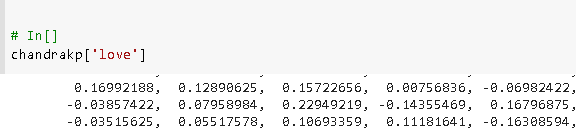
\includegraphics[width=7cm]{figures/1174079/5/8.png}
			\centering
			\caption{Praktek 1.1}
		\end{figure}
		\item Pada gambar ini Vektor faith memliki nilai 0.26 , tidak jauh dengan vektor love yang berarti kata ini bisa satu kategori
		\hfill\break
		\lstinputlisting[firstline=17, lastline=17]{src/1174079/5/1174079.py}
		\begin{figure}[H]
			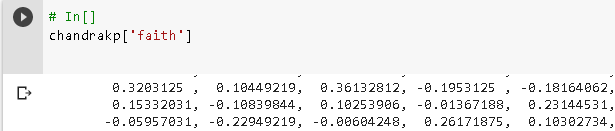
\includegraphics[width=7cm]{figures/1174079/5/9.png}
			\centering
			\caption{Praktek 1.2}
		\end{figure}
		\item vektor fall sayangnya hanya mempunyai poin negatif 0.04 yang berarti tidak bisa satu kategori dengan love dan faith
		\hfill\break
		\lstinputlisting[firstline=19, lastline=19]{src/1174079/5/1174079.py}
		\begin{figure}[H]
			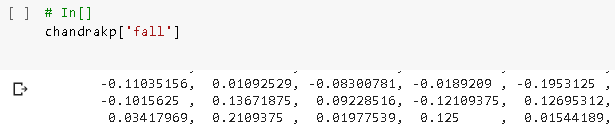
\includegraphics[width=7cm]{figures/1174079/5/10.png}
			\centering
			\caption{Praktek 1.3}
		\end{figure}
		\item vektor sick memiliki nilai yang sangat jauh sekali dengan yang lainnya yaitu 1.8 yang berarti tidak satu kategori dengan love, faith maupun fall.
		\hfill\break
		\lstinputlisting[firstline=21, lastline=21]{src/1174079/5/1174079.py}
		\begin{figure}[H]
			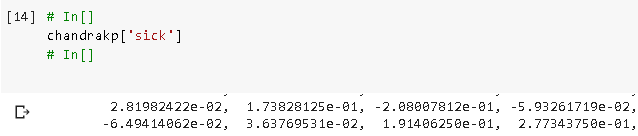
\includegraphics[width=7cm]{figures/1174079/5/11.png}
			\centering
			\caption{Praktek 1.4}
		\end{figure}
		\item vektor clear memiliki nilai yang sangat jauh sekali dengan yang lainnya yaitu-2,44 sangat jauh dari vektor fall sehingga tidak bisa satu kategori.
		\hfill\break
		\lstinputlisting[firstline=23, lastline=23]{src/1174079/5/1174079.py}
		\begin{figure}[H]
			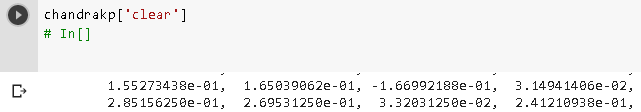
\includegraphics[width=7cm]{figures/1174079/5/12.png}
			\centering
			\caption{Praktek 1.5}
		\end{figure}
		\item vektor shine memiliki nilai -0.12 sayangnya tidak mendekati vektor manapun. 
		\hfill\break
		\lstinputlisting[firstline=25, lastline=25]{src/1174079/5/1174079.py}
		\begin{figure}[H]
			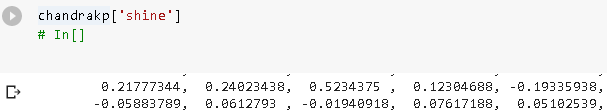
\includegraphics[width=7cm]{figures/1174079/5/13.png}
			\centering
			\caption{Praktek 1.6}
		\end{figure}
		\item Vektor bag mempunyai nilai identitas -0.03 yang dekat dengan salah satu vektor yaitu vektor fall. disini mesin mulai memahami bahwa kedua kategori ini bisa dijadikan satu kategori.
		\hfill\break
		\lstinputlisting[firstline=27, lastline=27]{src/1174079/5/1174079.py}
		\begin{figure}[H]
			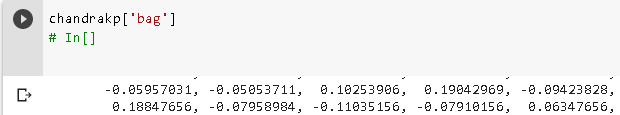
\includegraphics[width=7cm]{figures/1174079/5/14.png}
			\centering
			\caption{Praktek 1.7}
		\end{figure}
		\item Vektor car mempunyai nilai 0.13 yang dekat dengan vektor love serta faith sehingga bisa dijadikan satu kategori.
		\hfill\break
		\lstinputlisting[firstline=29, lastline=29]{src/1174079/5/1174079.py}
		\begin{figure}[H]
			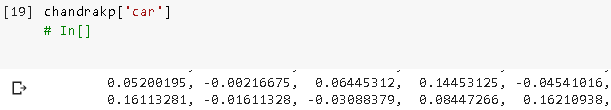
\includegraphics[width=7cm]{figures/1174079/5/15.png}
			\centering
			\caption{Praktek 1.8}
		\end{figure}
		\item Vektor wash mempunyai nilai sebesar 9.46 yang jauh sekali perbedaanya dengan vektor lain.
		\hfill\break
		\lstinputlisting[firstline=31, lastline=31]{src/1174079/5/1174079.py}
		\begin{figure}[H]
			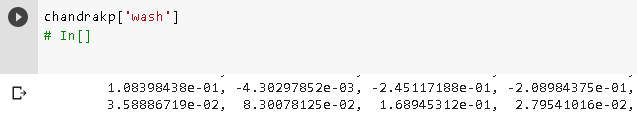
\includegraphics[width=7cm]{figures/1174079/5/16.png}
			\centering
			\caption{Praktek 1.9}
		\end{figure}
		\item Vektor motor mempinyai nilai identitas sebesar 5.73 yang dekat dengan nilai vektor wash.
		\hfill\break
		\lstinputlisting[firstline=33, lastline=33]{src/1174079/5/1174079.py}
		\begin{figure}[H]
			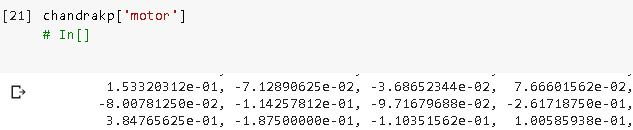
\includegraphics[width=7cm]{figures/1174079/5/17.png}
			\centering
			\caption{Praktek 1.10}
		\end{figure}
		\item Vektor cycle mempunyai nilai identitas sebesar 0.04
		\hfill\break
		\lstinputlisting[firstline=35, lastline=35]{src/1174079/5/1174079.py}
		\begin{figure}[H]
			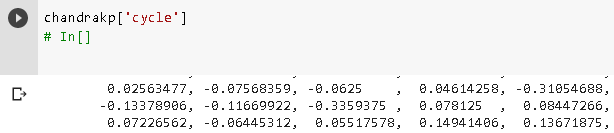
\includegraphics[width=7cm]{figures/1174079/5/18.png}
			\centering
			\caption{Praktek 1.11}
		\end{figure}
		\item berikut merupakan kesimpulan dari similaritas kata kata yang telah di olah menjadi matrix.
		Dapat disimpulkan bahwa:
		\begin{itemize}
		\item Untuk Love dan faith hasilnya adalah 37 
		\item Untuk Love dan fall hasilnya adalah 11
		\item Untuk Love dan clear hasilnya adalah 6
        \item Untuk Love dan shine hasilnya adalah 20
		\item Untuk Love dan bag hasilnya adalah 7
		\item Untuk Love dan car hasilnya adalah 8
		\item Untuk Love dan wash hasilnya adalah 11
		\item Untuk Love dan motor hasilnya adalah 8
		\item Untuk Love dan wash hasilnya adalah 5
		\end{itemize}
		Data diatas menggambarkan bahwa mesin sudah mengerti bahwa kata faith dan love yang artinya cinta serta kepercayaan merupakan satu kategori

		\hfill\break	
		\lstinputlisting[firstline=37, lastline=55]{src/1174079/5/1174079.py}
		\begin{figure}[H]
			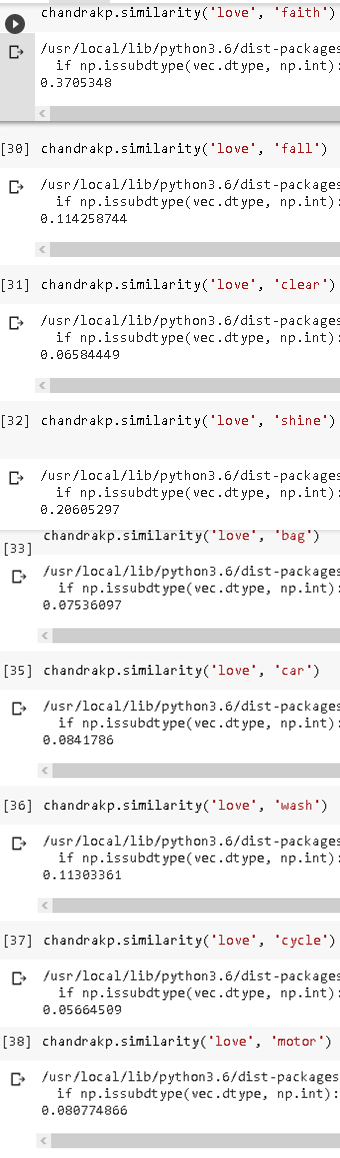
\includegraphics[width=7cm]{figures/1174079/5/19.png}
			\centering
			\caption{Praktek 1.12}
		\end{figure}
	\end{itemize}
	\item Jelaskan dengan kata dan ilustrasi fungsi dari extract words dan PermuteSentences
	\hfill\break
	ExtractWords adalah suatu function yang digunakan untuk memanipulasi data seperti menambahkan atau menghapuskan, berikut contohnya.
		\begin{figure}[H]
			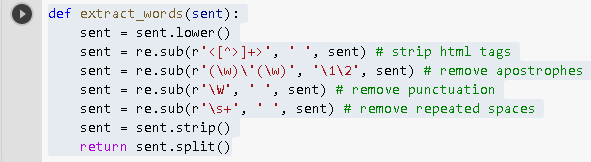
\includegraphics[width=7cm]{figures/1174079/5/20.png}
			\centering
			\caption{Praktek 2}
		\end{figure}
		\hfill\break
		PermuteSentences adalah class yang dipakai untuk melakukan randomnisasi data. 
		\begin{figure}[H]
			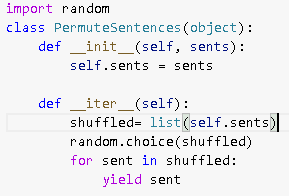
\includegraphics[width=7cm]{figures/1174079/5/21.png}
			\centering
			\caption{Praktek 2}
		\end{figure}

	\item Jelaskan fungsi dari librari gensim TaggedDocument dan Doc2Vec disertai praktek pemakaiannya.
	\hfill\break
	Doc2vec adalah suatu algoritma unsupervised yang digunakan untuk generate data berupa vektor seperti dokumen,kalimat,paragraf. Lalu TaggedDocument itu merupakan suatu function Doc2Vec yang dipakai untuk menampilkan kata yang diinginkan.

		\begin{figure}[H]
			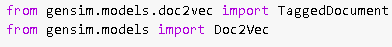
\includegraphics[width=7cm]{figures/1174079/5/22.png}
			\centering
			\caption{Praktek 3}
		\end{figure}
	\item Jelaskan dengan kata dan praktek cara menambahkan data training dari file yang dimasukkan kepada variabel dalam rangka melatih model doc2vac.
	\hfill\break
	
		\begin{figure}[H]
			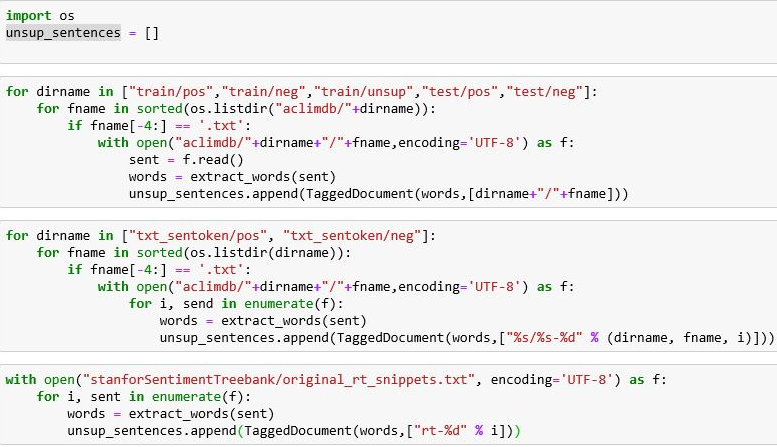
\includegraphics[width=7cm]{figures/1174079/5/23.png}
			\centering
			\caption{Praktek 4}
		\end{figure}
		
	\item Jelaskan dengan kata dan praktek kenapa harus dilakukan pengocokan dan pembersihan data.
	\hfill\break
	Pengocokan perlu untuk dilakukan supaya hasil yang didapat lebih akurat. Lalu Pembersihan data digunakan untuk menghapus data yang tidak diinginkan seperti spasi dan juga data noisy. 
		\begin{figure}[H]
			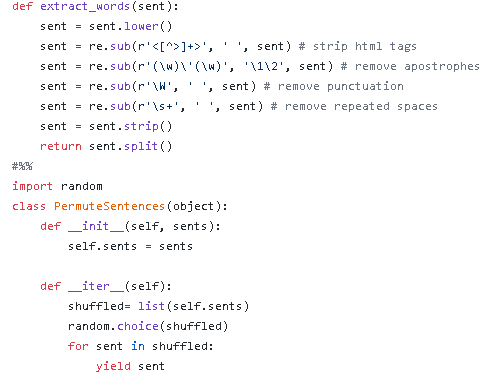
\includegraphics[width=7cm]{figures/1174079/5/24.png}
			\centering
			\caption{Praktek 5}
		\end{figure}
	\item Jelaskan dengan kata dan praktek kenapa model harus di save dan kenapa temporari training harus dihapus.
	\hfill\break
	Model disave agar nantinya kita mudah untuk mengedit atau menguji filenya kembali. Temporari training adalah data training yang telah kita jalankan sebelumnya, namun karena sudah kita buat modelnya dan juga untuk menghemat daya memori maka penghapusan data temporari training dirasa perlu untuk menghindari lag atau kejadian yang tidak diinginkan.
		\lstinputlisting[firstline=114, lastline=115]{src/1174079/5/1174079.py}
			
	\item Jalankan dengan kata dan praktek maksud dari infer code.
	\hfill\break
	Infer vektor dipakai untuk menhitung vektor dari dokumen atau kata yang diberikan
		\begin{figure}[H]
			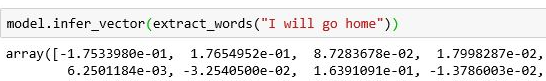
\includegraphics[width=7cm]{figures/1174079/5/26.png}
			\centering
			\caption{Praktek 7}
		\end{figure}

	\item Jelaskan dengan praktek dan kata maksud dari cosine similarity.
	Cosine similarity dipakai untuk melihat nilai kesamaan dari suatu paragraf atau kalimat yang kita berikan. apakah satu kategori atau tidaknya.
	\hfill\break
	
		\begin{figure}[H]
			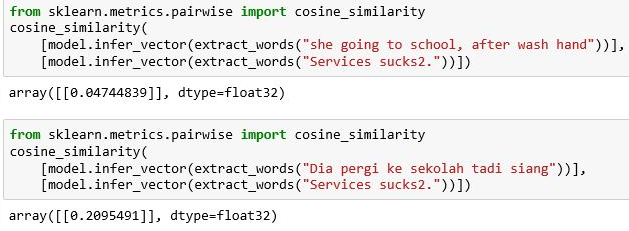
\includegraphics[width=7cm]{figures/1174079/5/27.png}
			\centering
			\caption{Praktek 8}
		\end{figure}
	\item Jelaskan dengan praktek score dari cross validation masing-masing metode.
	\lstinputlisting[firstline=136, lastline=158]{src/1174079/5/1174079.py}	
\end{enumerate}
\subsection{Penangan Error}
\begin{enumerate}
	\item word falla not in vocabulary
	\hfill\break
		\begin{figure}[H]
			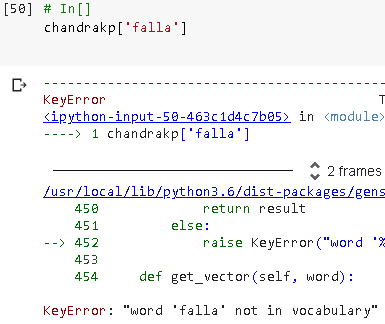
\includegraphics[width=7cm]{figures/1174079/5/error.png}
			\centering
			\caption{word falla not in vocabulary}
		\end{figure}
	\item Jenis error
	\begin{itemize}
		\item word falla not in vocabulary
	\end{itemize}
	\item Cara Penanganan
	\hfill\break
	typo, perbaiki
\end{enumerate}
\subsection{Bukti Tidak Melakukan Plagiat}
\hfill\break
\begin{figure}[H]
	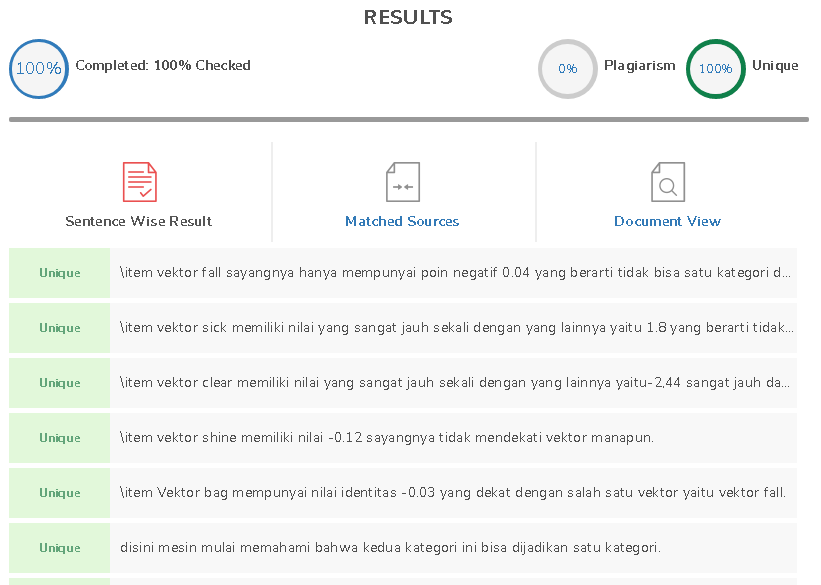
\includegraphics[width=4cm]{figures/1174079/5/plagiat.png}
	\centering
	\caption{Bukti Tidak Melakukan Plagiat}
\end{figure}

\subsection{Link Youtube}
https://youtu.be/YWgD7jAeT8A